%Copyright Page
\thispagestyle{empty}

\noindent 联系作者/获取更新
\begin{tabbing}
	作者邮箱\qquad \= \url{loniceras@163.com} \\
	获取更新 \> \url{https://github.com/loniceras/foundation_of_physical_chemistry}
\end{tabbing}

\vspace*{\baselineskip}
\noindent 建议的BibTeX信息
\begin{verbatim}
@book{Lonicera21,
    author={栀子忍冬},
    title={物理化学基础(v0.1)},
    year={2021},
    url={https://github.com/loniceras/foundation_of_physical_chemistry}
}
\end{verbatim}

\vspace*{\baselineskip}
\noindent 版本信息 (当前: v0.1)
\begin{tabbing}
	版本号\qquad \= 发布时间\qquad \= 主要修订内容 \\
	v0.1 \> 21.08.10 \> 初始版本 \\
\end{tabbing}

\vspace*{\baselineskip}
\noindent LaTeX模板信息
\vspace*{\topsep}\\
\noindent 本作品采用ElegantLaTeX系列模板的ElegantBook 4.1. 更多信息可访问项目官网 \url{https://elegantlatex.org} 和项目GitHub页面 \url{https://github.com/ElegantLaTeX}.

\vspace*{8cm}
\begin{window}[0,l,{\includegraphics{002_by_nc_sa.eps}},{}]
	\noindent 本作品采用知识共享署名-非商业性使用-相同方式共享 4.0 国际许可协议进行许可. 访问链接 \url{https://creativecommons.org/licenses/by-nc-sa/4.0} 查看该许可协议.
\end{window}